\documentclass[10pt,twoside,a4paper]{article}

\usepackage{fancyhdr}

\usepackage{lastpage}       % ``n of m'' page numbering
\usepackage{lscape}         % Makes landscape easier

\usepackage{verbatim}       % Verbatim blocks
\usepackage{listings}       % Source code listings
\usepackage{epsfig}         % Embed encapsulated postscript
\usepackage{array}          % Array environment
\usepackage{array}          % Array environment
\usepackage{enumitem}       % Required by Tom Johnson's exam question header

\usepackage{hhline}         % Horizontal lines in tables
\usepackage{siunitx}        % Correct spacing of units
\usepackage{amsmath}        % American Mathematical Society
\usepackage{amssymb}        % Maths symbols
\usepackage{amsthm}         % Theorems

\usepackage{ifthen}         % Conditional processing in tex

\usepackage[skip=0.5cm]{parskip}

\usepackage[top=3cm,
            bottom=3cm,
            inner=2cm,
            outer=2cm]{geometry}


% If you have any additional \usepackage commands, or other
% macros or directives, put them here.  Remember not to edit
% files in the template directory because any changes will
% be overwritten when template updates are issued.
\usepackage{float,graphicx}
\usepackage{amsmath}
\usepackage{amssymb}
\usepackage{caption}

\usepackage[absolute,overlay]{textpos}

\newcolumntype{C}{>$c<$}
\graphicspath{ {./images/} }

\newcommand{\notimplies}{%
  \mathrel{{\ooalign{\hidewidth$\not\phantom{=}$\hidewidth\cr$\implies$}}}}
\newcommand{\Mod}[1]{\ (\mathrm{mod}\ #1)}
\newcommand{\Z}{\mathbb{Z}}
\newcommand{\R}{\mathbb{R}}
\newcommand{\Q}{\mathbb{Q}}
\newcommand{\N}{\mathbb{N}}


\title{Delay-Tolerant Link-State Routing}
\author{Ben Andrew, ba405\\Magdalene College}
\date{\today}


\begin{document}
\maketitle


\section{Declaration of Originality}

\section{Proforma}

\section{Table of Contents}

\section{Introduction}

\section{Preparation}

\section{Implementation}

\subsection{Repository Overview}

\begin{verbatim}
dtlsr                        Root
|- configs                   CORE config files
|- include                   Include directory
|  |- algorithm
|  |- network
|  "- process
|- src                       Source directory
|  |- algorithm
|  |- network
|  "- process
|- tests                     Unit tests directory
|  |- algorithm
|  |- network
|  "- process
|- tools                     Custom development tools
"- core-py                   Custom CORE scripts
\end{verbatim}

\texttt{algorithm} contains pure algorithms and data structures, for example graph, graph searching, and heap implementations.

\texttt{network} contains functionality for socket manipulation, and sending data over the network.

\texttt{process} contains funtionality for interacting with both CORE and the Unix OS, for example retreiving node information, logging, and manipulating the Unix routing table.

The project was implemented almost entirely in C, with CORE-specific scripts in Python. I used the CMake build system and Check unit testing framework.


\subsection{CORE Background}

The Common Open Research Emulator (CORE) is a network emulator that models nodes as lightweight Unix virtual machines, complete with filesystems and network interfaces.

\begin{minipage}{1\textwidth} \centering
		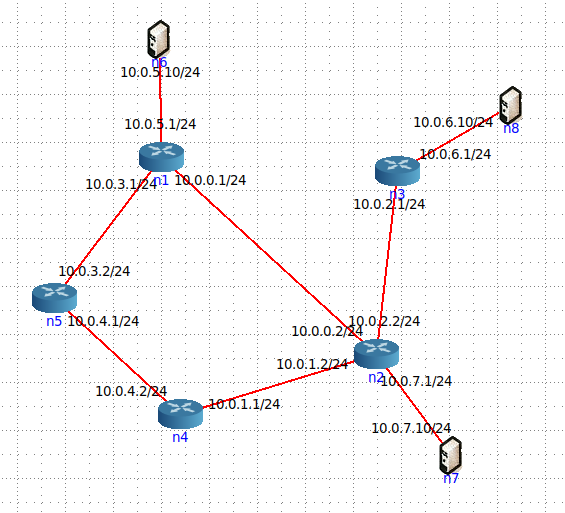
\includegraphics[width=0.6\textwidth]{6-core}
		\captionof{figure}{Example emulated network in the CORE GUI, showing routers and hosts.}
	\end{minipage}

Programs can be written for these nodes and run as Unix processes via a Python API. These processes are then able to send and receive data through the emulated network via standard Unix socket programming. The emulated routers contain default routing protocol implementations, such as OSPFv2 and v3 from the Quagga protocol suite, which can be disabled and replaced by custom implementations. As well as this, standard network testing tools like \texttt{iperf} can be run on emulated endpoint hosts, making testing and evaluation of the network surprisingly simple.

Link properties can be programmatically customised through the Python API, with properties including bandwidth, delay, loss, and jitter. This will aid greatly in evaluation, for example simulating network partitions.

One limitation is that CORE operates in real-time using the OS's clock, and thus the performance of the simulated network is somewhat dependent on the performance of the machine it's being run on. I will therefore be taking great care to create a reliable and statistically sound testing environment, for example setting processor priority, not running other programs, and taking baseline measurements to compare against.

\subsection{Link-State Routing Design}

The subset of OSPF that I implemented is split into two programs, \texttt{heartbeat} and \texttt{dtlsr}. Routers run both programs, and hosts run only \texttt{heartbeat}.

\texttt{heartbeat} sends periodic heartbeat messages to all neighbouring nodes, notifying them that the connecting link is still up. The message is received by \texttt{dtlsr}.

\texttt{dtlsr} implements the bulk of the protocol. It maintains the link-state graph representation of the network, manipulates the node's routing table, and sends link-state announcements (LSAs) in response to detected changes in the network.

These changes are detected in one of three ways:
\begin{enumerate}
	\item
	A heartbeat message is received from a neighbour with a DOWN link.
	
	\item
	A heartbeat is not received in time from a neighbour with an UP link.
	
	\item
	An LSA is received from a neighbour.
\end{enumerate}

Both programs lend themselves to an event-driven design, and so I used file descriptors multiplexed with the \texttt{select} Unix call to detect and respond to events. Timer file descriptors trigger when they expire and sending socket file descriptors trigger when data arrives.

Heartbeats and LSAs are recieved on sockets with distinct ports, allowing them to be differentiated easily. While CORE supports IPv6 routing, I restricted myself to IPv4 to reduce unnecessary implementation complexity.

\subsubsection{Delay-Tolerant Modifications}

For the delay-tolerant version, \texttt{dtlsr} can be recompiled with the \texttt{-DDTLSR} flag active, keeping \texttt{heartbeat} identical. \texttt{dtlsr} maintains the same implementation design decisions as above.

TODO: actually implement DTLSR and say what I did. Link status history, etc.



\section{Evaluation}

\section{Conclusions}

\section{Bibliography}

\section{Appendices}

\section{Index}

\section{Project Proposal}



\end{document}





























